\documentclass{standalone}
\usepackage{pgfplots}


\begin{document}

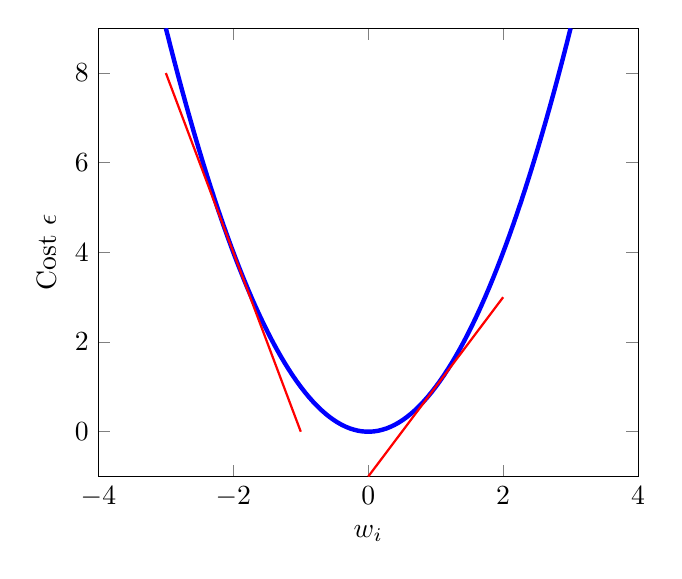
\begin{tikzpicture}
\begin{axis}[xmax=4,xmin=-4,ymax=9, ymin=-1, samples=100, xlabel={$w_i$}, ylabel={Cost $\epsilon$}, title style={font=\huge}]
  % TODO: remove axes

%  \addplot[domain=-9:9, gray] (x, 0);
%  \addplot[domain=-9:9, gray] (0, x);
  \addplot[domain=-3:3, blue, ultra thick] (x, x*x);

  \addplot[domain=0:2, red, thick] (x, 2*1*x-1);
  \addplot[domain=-3:-1, red, thick] (x, 2*-2*x-4);

% x^2
% find tangent at (1, 1)
% slope of tangent = 2x = 2*1
% intercept of tangent = b = -1

% find tangent at (-2, 4)
% slope of tangent = 2*-2
% intercept = b = -8
% -4*-2 + b = 0

\end{axis}
\end{tikzpicture}

\end{document}